\documentclass[runningheads]{llncs}



\usepackage{enumitem}


\usepackage{color}

\usepackage{graphicx}
\usepackage{tikz}
\usepackage{calc}
\usepackage{array}

\usepackage{amsmath, amssymb}
\DeclareMathOperator*{\argmin}{arg\,min}

\usepackage{graphbox}
\usepackage{wasysym}

\usetikzlibrary{automata,arrows}

\usepackage{comment}

\usepackage{wrapfig}

\usepackage{hyperref}


\title{Counting infinitely by Oritatami co-transcriptional folding}

%\titlerunning{}
\author{
Kohei Maruyama\inst{1}\thanks{Primary corresponding author (\email{k.maruyama@uec.ac.jp})} \and
Shinnosuke Seki\inst{1}\thanks{Secondary corresponding author (\email{s.seki@uec.ac.jp})}
}
\institute{
The University of Electro-Communications, 
%Graduate School of Informatics and Engineering, 
1-5-1 Chofugaoka, Chofu, Tokyo, 1828585, Japan \\
}

\begin{document}

\maketitle

\begin{abstract}
abstract
\end{abstract}

%------------------------------------------------------
	\section{Introduction}
%------------------------------------------------------
Our body consists many proteins which is based on genetic sequence in DNA.
DNA sequence has to be copied in order to make proteins because DNA is in cell nucleus.
It is copied to RNA (and its sequence is called \textit{transcript}) by a RNA polymerase and delivered to out of nucleus.
A transcript consists four types nucleobases A, U, G, and C, and a nucleobase are called \textit{bead}
Moreover, they form hydrogen bonds mainly between A and U, and between G and C, then they begin to form at the same time synthesizing.
Once the bead is fixed after that it can not change the position.
By repeating this method, transcript form a 3D shape.

A shape of RNA depends on the DNA sequence.
Geary, Rothemund, and Andrsen have succeeded in experimentally making 2D RNA tiles (Fig.\ref{fig:rna_origami}) by repeatedly copying a specific DNA sequence \cite{GearyRothemundAndersen2014}.
Then, Oritatami System was designed as a mathematical model that the process of RNA production and Fig.\ref{fig:origami_on_oritatami} is the 2D RNA tile which is represented on Oritatami System.


\begin{figure}[tb]
\centering
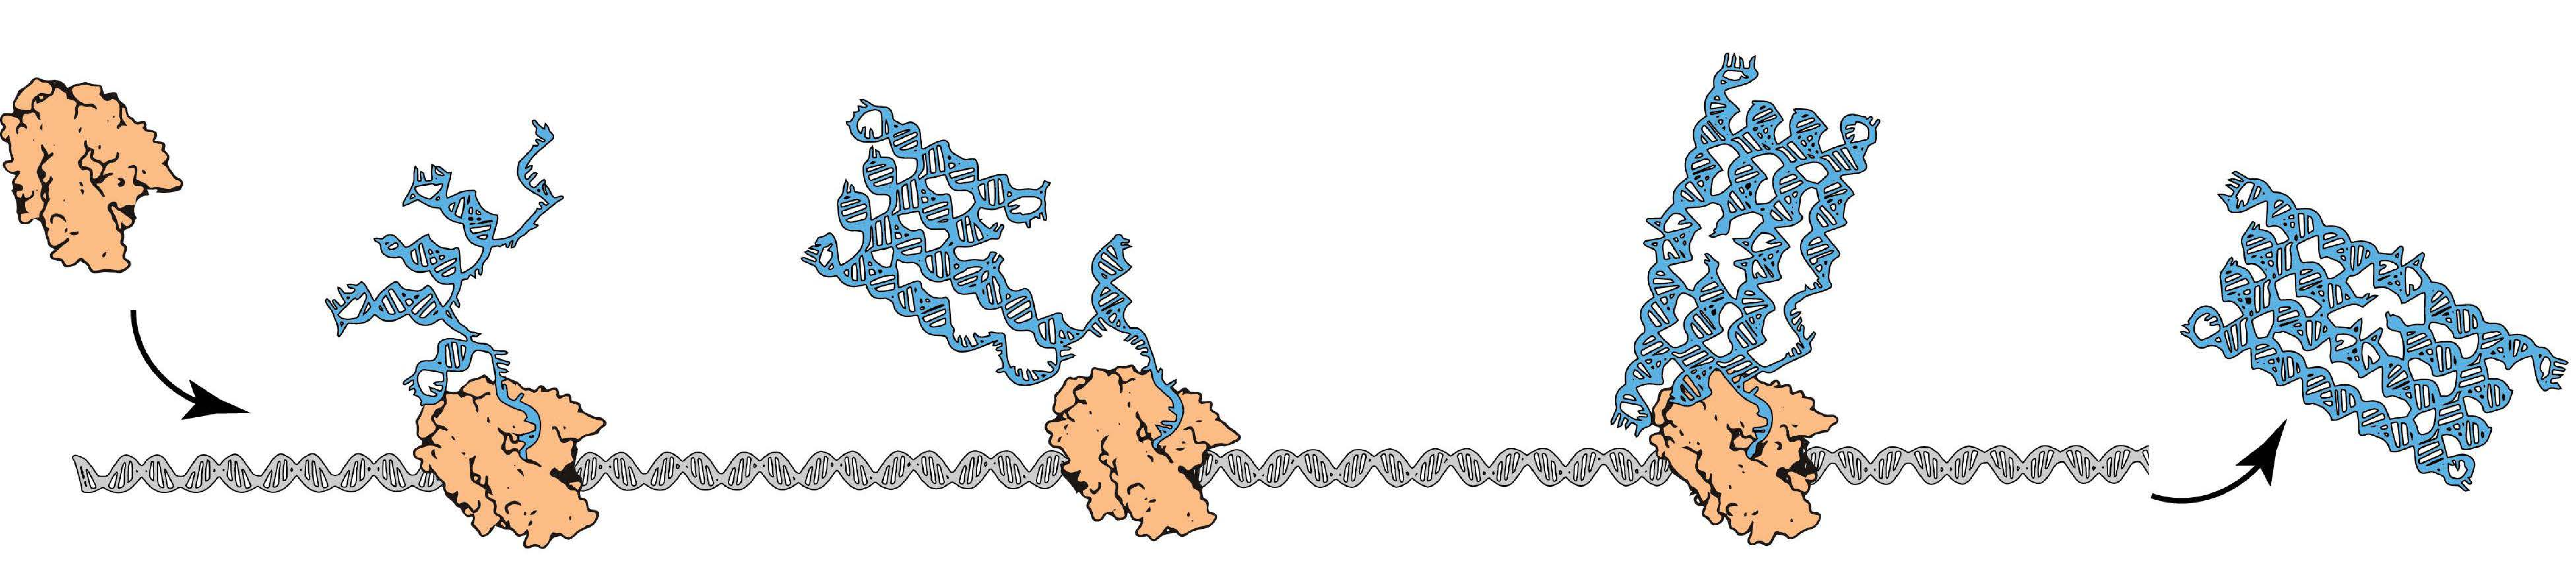
\includegraphics[width=\linewidth]{fig/rna_origami.pdf}
\caption{
A generated and stabilized 2D RNA tile from DNA
}
\label{fig:rna_origami}
\end{figure}

\begin{figure}[tb]
\centering
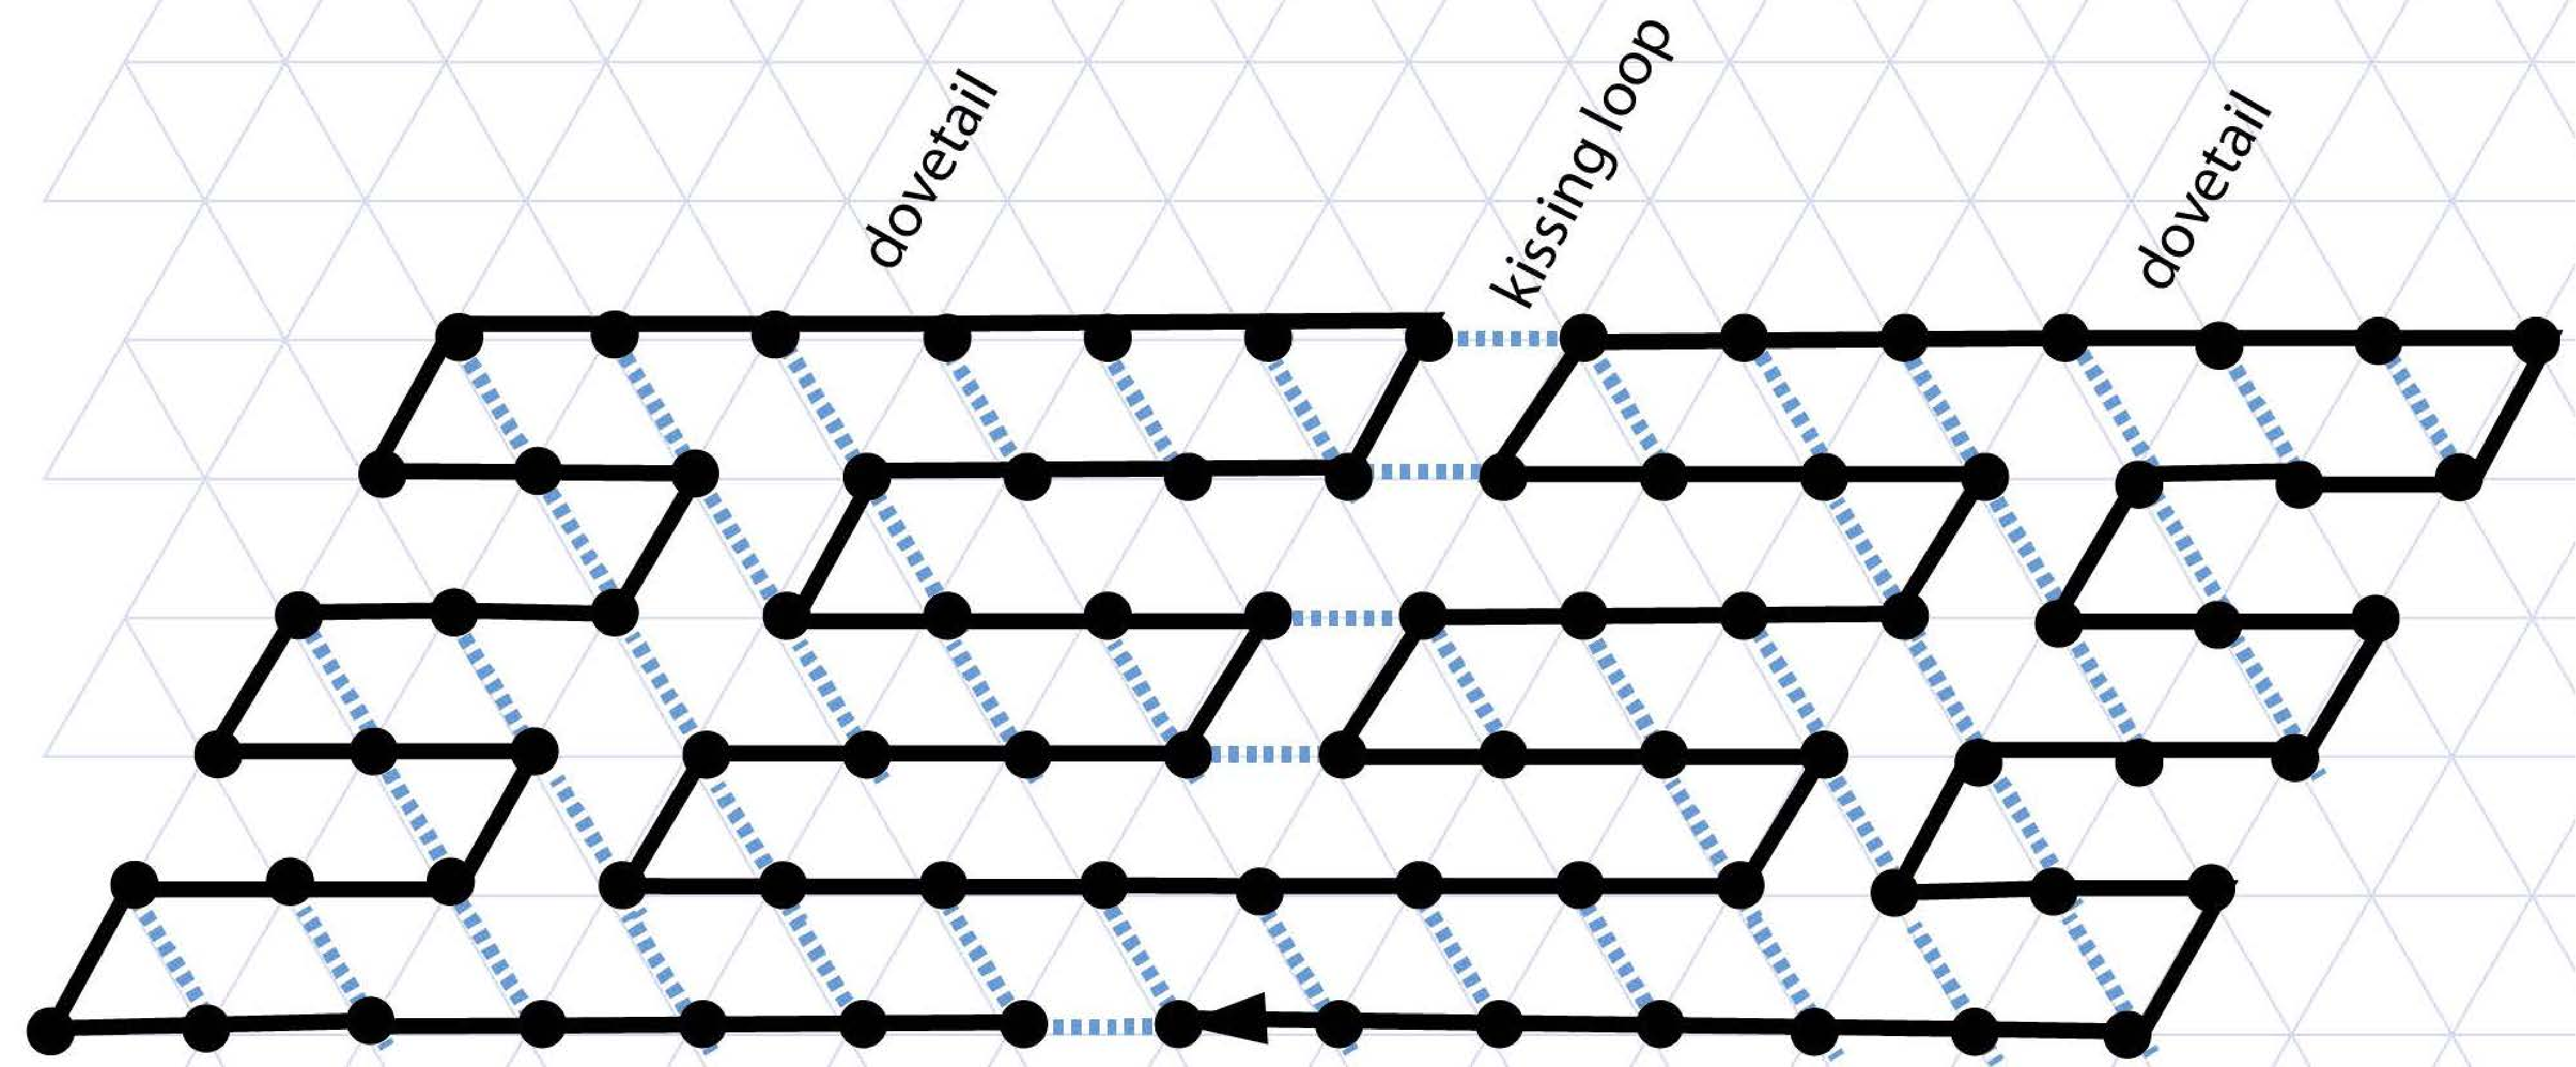
\includegraphics[width=\linewidth]{fig/origami_oritatami.pdf}
\caption{
The represented 2D RNA tile on Oritatami System
}
\label{fig:origami_on_oritatami}
\end{figure}



%------------------------------------------------------
	\section{Preliminaries}
%------------------------------------------------------

%copy from TAMC2019 paper

Let $\Sigma$ be a finite set of types of abstract molecules, or \textit{beads}. 
A bead of type $a \in \Sigma$ is called an $a$-bead. 
By $\Sigma^*$ and $\Sigma^\omega$, we denote the set of finite sequences of beads and that of one-way infinite sequences of beads, respectively. 
The empty sequence is denoted by $\lambda$. 
Let $w = b_1 b_2 \cdots b_n \in \Sigma^*$ be a sequence of length $n$ for some integer $n$ and bead types $b_1, \ldots, b_n \in \Sigma$. 
The \textit{length} of $w$ is denoted by $|w|$, that is, $|w| = n$. %ここから要らない?↓やっぱり要る
For two indices $i, j$ with $1 \le i \le j \le n$, we let $w[i..j]$ refer to the subsequence $b_i b_{i+1} \cdots b_{j-1}b_j$; if $i = j$, then $w[i..i]$ is simplified as $w[i]$. 
For $k \ge 1$, $w[1..k]$ is called a \textit{prefix} of $w$. 

Oritatami systems fold their transcript, which is a sequence of beads, over the triangular grid graph $\mathbb{T} = (V, E)$ cotranscriptionally. %↓
We designate one point in $V$ as the origin $O$ of $\mathbb{T}$. 
For a point $p \in V$, let $\hexagon_p^d$ denote the set of points which lie in the regular hexagon of radius $d$ centered at the point $p$. 
Note that $\hexagon_p^d$ consists of $3d(d+1)+1$ points. %←
A directed path $P = p_1 p_2 \cdots p_n$ in $\mathbb{T}$ is a sequence of \textit{pairwise-distinct} points $p_1, p_2, \ldots, p_n \in V$ such that $\{p_i, p_{i+1}\} \in E$ for all $1 \le i < n$. 
Its $i$-th point is referred to as $P[i]$. 
Now we are ready to abstract RNA single-stranded structures in the name of conformation. 
A \textit{conformation} $C$ (over $\Sigma$) is a triple $(P, w, H)$ of a directed path $P$ in $\mathbb{T}$, $w \in \Sigma^*$ of the same length as $P$, and a set of h-interactions $H \subseteq \bigl\{\{i, j\} \bigm| 1 \le i, i+2 \le j, \{P[i], P[j]\} \in E \bigr\}$. 
This is to be interpreted as the sequence $w$ being folded along the path $P$ in such a manner that its $i$-th bead $w[i]$ is placed at the $i$-th point $P[i]$ and the $i$-th and $j$-th beads are bound (by a hydrogen-bond-based interaction) if and only if $\{i, j\} \in H$. 
The condition $i+2 \le j$ represents the topological restriction that two consecutive beads along the path cannot be bound. 
The \textit{length} of $C$ is defined to be the length of its transcript $w$ (that is, equal to the length of the path $P$). 
A \textit{rule set} $R \subseteq \Sigma \times \Sigma$ is a symmetric relation over $\Sigma$, that is, for all bead types $a, b \in \Sigma$, $(a, b) \in R$ implies $(b, a) \in R$.
A bond $\{i, j\} \in H$ is \textit{valid with respect to $R$}, or simply $R$-valid, if $(w[i], w[j]) \in R$. 
This conformation $C$ is \textit{$R$-valid} if all of its bonds are $R$-valid. %↓
For an integer $\alpha \ge 1$, $C$ is \textit{of arity $\alpha$} if it contains a bead that forms $\alpha$ bonds but none of its beads forms more. 
By $\mathcal{C}_{\le \alpha}(\Sigma)$, we denote the set of all conformations over $\Sigma$ whose arity is at most $\alpha$; its argument $\Sigma$ is omitted whenever $\Sigma$ is clear from the context. 

The oritatami system grows conformations by an operation called elongation. 
Given a rule set $R$ and an $R$-valid conformation $C_1 = (P, w, H)$, we say that another conformation $C_2$ is an elongation of $C_1$ by a bead $b \in \Sigma$, written as $C_1 \xrightarrow{R}_b C_2$, if $C_2 = (P p, wb, H \cup H')$ for some point $p \in V$ not along the path $P$ and set $H' \subseteq \bigl\{ \{i, |w|+1\} \bigm| 1 \le i < |w|, \{P[i], p\} \in E, (w[i], b) \in R \bigr\}$ of bonds formed by the $b$-bead; this set $H'$ can be empty. 
Note that $C_2$ is also $R$-valid. 
This operation is recursively extended to the elongation by a finite sequence of beads as: for any conformation $C$, $C \xrightarrow{R}_\lambda^* C$; and for a finite sequence of beads $w \in \Sigma^*$ and a bead $b \in \Sigma$, a conformation $C_1$ is elongated to a conformation $C_2$ by $wb$, written as $C_1 \xrightarrow{R}_{wb}^* C_2$, if there is a conformation $C'$ that satisfies $C_1 \xrightarrow{R}_w^* C'$ and $C' \xrightarrow{R}_b C_2$. 

An \textit{oritatami system} (OS) $\Xi = (\Sigma, R, \delta, \alpha, \sigma, w)$ is composed of
\begin{itemize}
\item a set $\Sigma$ of bead types, 
\item a rule set $R \subseteq \Sigma \times \Sigma$, 
\item a positive integer $\delta$ called the \textit{delay}, 
\item a positive integer $\alpha$ called the \textit{arity}, %←arityの行だけ要らない?
\item an initial $R$-valid conformation $\sigma \in C_{\le \alpha}(\Sigma)$ called the \textit{seed}, whose first bead is assumed to be at the origin $O$ without loss of generality, 
\item a (possibly infinite) \textit{transcript} $w \in \Sigma^* \cup \Sigma^\omega$, which is to be folded upon the seed by stabilizing beads of $w$ one at a time so as to minimize energy collaboratively with the succeeding $\delta{-}1$ nascent beads. 
\end{itemize}
%
The energy of a conformation $C = (P, w, H)$, denoted by $\Delta G(C)$, is defined to be ${-}|H|$; the more bonds a conformation has, the more stable it gets. 
The set $\mathcal{F}(\Xi)$ of conformations \textit{foldable} by the system $\Xi$ is recursively defined as: the seed $\sigma$ is in $\mathcal{F}(\Xi)$; and provided that an elongation $C_i$ of $\sigma$ by the prefix $w[1..i]$ be foldable (i.e., $C_0 = \sigma$), its further elongation $C_{i+1}$ by the next bead $w[i+1]$ is foldable if 
\begin{equation}\label{eq:OS_CF}
C_{i+1} \in \argmin_{
\substack{
C \in \mathcal{C}_{\le \alpha} s.t. \\
C_i \xrightarrow{R}_{w[i+1]}C \\
}
}
\min \Bigl\{ \Delta G(C') \Bigm|
C \xrightarrow{R}^*_{w[i+2...i+k]}C', k\le \delta, C' \in \mathcal{C}_{\le \alpha}
\Bigr\}.
\end{equation}
%
Then we say that the bead $w[i+1]$ and the bonds it forms are \textit{stabilized} according to $C_{i+1}$. 
The easiest way to understand this stabilization process should be the video available at \href{https://www.dailymotion.com/video/x3cdj35}{\tt https://www.dailymotion.com/video/x3cdj35}, in which the Turing universal oritatami system by Geary et al. \cite{GeMeScSe2018}, whose delay is 3, is running. 
Note that an arity-$\alpha$ oritatami system cannot fold any conformation of arity larger than $\alpha$. %←
A conformation foldable by $\Xi$ is \textit{terminal} if none of its elongations is foldable by $\Xi$. 
%The oritatami system $\Xi$ is \textit{deterministic} if for all $i \ge 0$, there exists at most one $C_{i+1}$ that satisfies \eqref{eq:OS_CF}. 
%A deterministic oritatami system folds into a unique terminal conformation. 
%An oritatami system with the empty rule set just folds into an arbitrary elongation of its seed nondeterministically. 
%Thus, the rule set is reasonably assumed non-empty. 

\section{Folding an infinite binary counter}

\subsection{General idea}
Basically, an folding process of counter is the same way as Geary et al \cite{counter2016}.
The construction proceeds in zig-zags.
Each pass is 3-rows thick and folds each part of the bead into a glider or turn module.
Each pass extends to straight while folding into glider and folds its last module folds into turn module and starts next pass.
The zig pass, folding from right to left, counts up in the current value of the counter.
The zag pass, folding from left to right, formats and copy to downward the value which the zig pass represents.

The module is semantically divided into 4 parts, called modules:
\begin{itemize}
\item Module F (beads 1--30): the Format module
\item Module L (beads 31--66): the Left-Turn module
\item Module H (bead 67--96): the Half-Adder module
\item Module R (bead 97--132): the Right-Turn module 
\end{itemize}

\subsubsection{Encoding}
The current value of the counter is encoded in standard binary with the most significant bit to the left.
Binary is encoded into a specific folding of the module F and H.
In zig pass, folding of module H corresponds to module F in a zag pass: namely H0 for 0, and H1 for 1.
In addition, start position of modules represents the carry: carry = 0 if module H starts to fold in the top row; carry = 1 if module H start to fold from the bottom row.
On the other hand in zag pass, folding of module F corresponding to module H in a zig pass: namely F0 for 0, and F1 for 1.

\subsubsection{In the zig pass ($\leftarrow$)}
Module H read from the row above the value encoded into folding in the module F during the previous zag-phase, and fold into a shape H00, H10, H01, H11.
H$xc$ is corresponding to the case where $x$ is the bit read in the row above and $c$ is the carry. 
In the zig pass module R, F, and L just propagate the carry value to the next.

When the zig pass reaches the left most part, module L collaborates with above turn module and it is folded turn module which reverses the folding direction for next zag pass except carry = 1.
At this time, if module L has a carry, folding of module L is glider and it go straight in order to expand bit width after that next module L turns to zag pass while folding turn module.
%H -> He1

\subsubsection{In the zag pass ($\rightarrow$)}
Module F read form the row above H$xc$, and fold into a shape F0, F1.
F$y$ is corresponding to the case where $y = (x + c)$ mod $2$.
There are no carry propagation and the module L, H, R fold into Lbc, Hn, Rb in this pass.

When the zag pass reaches the right most part. module R collaborates with above turn module and it is folded turn module which reverses the folding direction for next zag pass.

\subsection{Example of folding}
Let's run an infinite counter from 1 bit width.

\subsubsection{The seed conformation}


\bibliographystyle{splncs03}
\bibliography{sofsem2020}
  
\end{document}
